\documentclass[tikz,border=2pt]{standalone}
\usepackage{amsmath}
\usetikzlibrary{arrows.meta}
\begin{document}
% Riley's controlled two-oven policy (Section 5.2): lambda(n) = 1.9 for all n, mu(n) = 2 for 1 <= n <= 4
% and mu(n) = 4 for n >= 5 (second oven switched on from five jobs on); birth-death chain on n = 0, 1, 2, ...
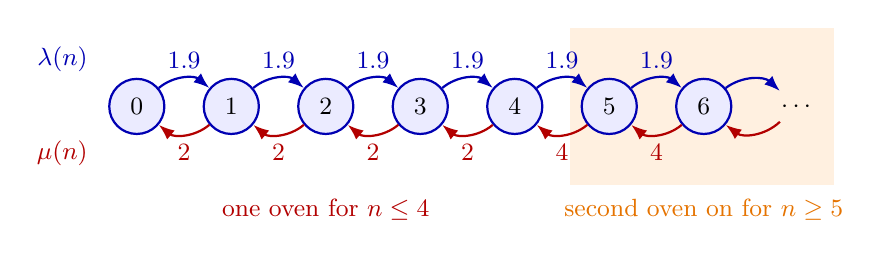
\begin{tikzpicture}[font=\small, >={Latex[length=2mm]},
  st/.style={circle, draw=blue!70!black, thick, fill=blue!8, minimum size=7mm, inner sep=0pt}]
  \def\d{1.2}
  \fill[orange!12] (\d*5-0.5,-1.0) rectangle (\d*7+0.45,1.0);
  \foreach \n in {0,...,6} \node[st] (s\n) at (\d*\n,0) {$\n$};
  \node (dots) at (\d*7,0) {$\cdots$};
  \foreach \n/\m in {0/1,1/2,2/3,3/4,4/5,5/6}
    \draw[->, thick, blue!70!black] (s\n) to[bend left=40] node[above] {$1.9$} (s\m);
  \draw[->, thick, blue!70!black] (s6) to[bend left=40] (dots);
  \foreach \n/\m/\r in {0/1/2,1/2/2,2/3/2,3/4/2,4/5/4,5/6/4}
    \draw[->, thick, red!70!black] (s\m) to[bend left=40] node[below] {$\r$} (s\n);
  \draw[->, thick, red!70!black] (dots) to[bend left=40] (s6);
  \node[blue!70!black, anchor=east] at (-0.5,0.6) {$\lambda(n)$};
  \node[red!70!black, anchor=east] at (-0.5,-0.6) {$\mu(n)$};
  % threshold: second oven on from n = 5
  \node[orange!90!black, anchor=north] at (\d*6,-1.05) {second oven on for $n\geq5$};
  \node[red!70!black, anchor=north] at (\d*2,-1.05) {one oven for $n\leq4$};
\end{tikzpicture}
\end{document}
